\documentclass{article}
\usepackage{graphicx} % Required for inserting images
\usepackage{amsmath}
\usepackage{amssymb}
\usepackage{floatrow}
\usepackage{changepage}
\usepackage{siunitx}

\title{Elliptical Filter Design}
\author{Name : Joel Anto Paul\\ Roll No : 210070037}

\begin{document}

\maketitle

\section{Theory behind Elliptical Filter}
\textbf{Why Elliptic filter?}\\
We prefer elliptic approximation to realise filters because, for a given order, the transition band is the smallest. This allows us to achieve the best approximation with the fewest resources. On the contrary we get very less phase control.
\subsection{Transfer Function}
The transfer function for an elliptic filter (or any type of FIR filter in general) is as follows:
\begin{equation*}
    |H(j\Omega)|^2 = \frac{1}{1+\epsilon_p^2U_N^2(w)};  w=\frac{\Omega}{\Omega_p}
\end{equation*}
where, N is the order of filter and $F_N$ is given by
\begin{equation*}
F_N^2(w)= 
\left\{
    \begin{array}{lr}
        cd(NuK_1,k_1)&\text{Elliptic}\\
        w^2 & \text{Butterworth} \\
        C_N(w), & \text{Chebyschev} \\        
    \end{array}
\right\}
\end{equation*}\\
Here,
$C_N$ is Chebyschev function and cd is a Jacobi elliptic function.\\
\hspace*{9mm} k (selectivity parameter) is defined as the ratio of passband to stopband frequency\\
\hspace*{9mm} $k_1$ (discrimination parameter) is defined as the ratio of $\epsilon_p$ and $\epsilon_s$
\begin{equation*}
    \epsilon_p = {\sqrt{(\frac{1}{1-\delta_1})^2-1}}
\end{equation*}
\begin{equation*}
    \epsilon_s = {\sqrt{(\frac{1}{\delta_2})^2-1}}
\end{equation*}
For the filter specifications provided to us we have  $\delta1=\delta2=0.15$ \\
\subsection{Elliptic Function}
Elliptic Functions are meromorphic and doubly periodic functions extendable to Complex plane.
There are total 3 types of elliptic functions, but here we are going to use only the first kind for designing Elliptic filter.
\begin{equation}
    \textbf{Elliptic Function of First Kind: }
    F(\phi,k) = \int_{0}^{\phi} \frac{\,d\theta}{\sqrt{1-k^2\sin^2(\theta)}} 
\end{equation}
k is also called the eccentricity or elliptical modulus.(This can be related to arc length finding integral of ellipse)\\
\\
We define another quantity K(k) as the complete elliptical integral of order 1.
\begin{equation}
    K(k) = F(\frac{\pi}{2},k)
\end{equation}
Also for further calculation we introduce k' = $\sqrt{1-k^2}$ 'complementary elliptical modulus, with following relation:
\begin{equation*}
    K(k') = K'(k)
\end{equation*}
For calculations in Matlab,we use same standard naming convention.

\subsection{Jacobi Elliptical Function}
There are total of 12 function represented as pq(z,k) where p,q $\in$ {s,c,d,n} and for p = q the value of function becomes trivially 1. Therefore total of 12 functions to study.\\
For making our elliptical filter we are focused only on cd(z,k) and sn(z,k).\\
These functions can be generated from theta functions, but here we will use Elliptical First Kind integral. We define z = F($\phi$,k) (from equation 1). We then find inverse of F($\phi$,k) with respect to $\phi$ and call it \textit{Jacobi Amplitude}.
\begin{equation*}
    \phi = amp(z,k)
\end{equation*}
\begin{equation}
    sn(z,k) = \sin(\phi) = \sin(amp(z,k))
\end{equation}
\begin{equation}
    cn(z,k) = \cos(\phi) = \cos(amp(z,k))
\end{equation}
\begin{equation}
    dn(z,k) = \frac{d}{dz}(\phi) = \frac{d}{dz}(amp(z,k))
\end{equation}
Equation 3, 4, 5 form the basis of Jacobi Elliptical Functions and rest 9 can formed from these 3 by following relation.
\begin{equation*}
    pq(z,k) = \frac{1}{qp(z,k)}
\end{equation*}
\begin{equation*}
    pq(z,k) = \frac{pr(z,k)}{qr(z,k)}; \text{where }r \in \{s,n,c,d\}
\end{equation*}
Here,  z is the arbitrary complex vector, and k is the elliptic modulli.\\
We will be using only the following 2 functions majorly : cd(z,k) and $sn^{-1}(u,k)$\\

\begin{equation*}
    cd(z,k) = cde(z/K,k)
\end{equation*}
\begin{equation*}
    sn(z,k) = sne(z/K,k)
\end{equation*}
\begin{equation*}
    v = asne(u,k) \text{ means v is solution of : } sn(v\cdot K,k) = u
\end{equation*}
(The above 3 equations are for equivalent matlab functions used)

\subsection{Parameters, Poles and Zeroes}
We already know how k and k' are evaluated section 2.1 . Now to kind Order:\\
\begin{equation}
    \textbf{Degree Equation : }N = ceil({\frac{K(k)\cdot K'(k_1)}{K'(k)\cdot K(k_1)}})
\end{equation}
N can be represented as 2l+r, where r $\in$ \{0,1\}\\
Now, because there is ceiling function,  so there will be some overdesign(meeting more that specified requirements) i.e. $|H(j\Omega)|$ will fall below $\delta_2$ before reaching stopband frequency as N is not exact integer without ceil. So we can change our specs to new value of k such that N comes out to be same exact integer without ceil. 

In matlab, this is done by using \textit{ellipdeg(N,k$_1$)}, this returns the value of k which satisfies the degree equation (6) for given value of N and K$_1$.\\
Now the value of k has been updated, and this value will be used further in design.\\
\textbf{Zeroes:} Zeroes of H(j$\Omega$) are poles of U$_N$($\Omega$).
Let us first define few things:
\begin{equation*}
    u_i = \frac{2i-1}{N}\text{ ; where } i \in {1,2,...,l}
\end{equation*}
\begin{equation*}
    \zeta_i = cd(u_i\cdot K(k),k) = \textit{cde}(u_i,k)
\end{equation*}
\begin{equation}
    U_N(\Omega) = (\Omega)^r\Pi_{i=1}^l\left[\left(\frac{\Omega^2-\zeta_i^2}{1-\Omega^2k^2\zeta_i^2}\right)\cdot\left(\frac{1-k^2\zeta_i^2}{1-\zeta_i^2}\right)\right]
\end{equation}
$U_N$ has total 2l poles therefore there are total of 2l zeroes of H(j$\Omega$), which are given by : 
\begin{equation}
    z_i = \frac{j}{k\zeta_i}\text{ ; where } i \in {1,2,...,l}
\end{equation}
Remaining zeroes are $z_i^*$ i.e. conjugates of $z_i$\\
\\
\textbf{Poles:}
\begin{equation*}
    U_N(\Omega) = \frac{\pm j}{\epsilon_p}
\end{equation*}
There are 2l+r i.e. N poles to $|H(j\Omega)|$\\
Let v $\in \mathbb{R}$ be a solution to $sn(jv\cdot N\cdot K(k),k)$ = j/$\epsilon_p$, therefore
\begin{equation}
    v = \frac{-j}{N\cdot K(k)}sn^{-1}(\frac{j}{\epsilon_p},k_1) = \frac{-j}{N}asne(\frac{j}{\epsilon_p},k_1)
\end{equation}
Poles are given by:
\begin{equation}
    p_i = jcd((u_i-jv)K(k),k) = jcde(u_i-jv,k)\text{ ,where } i\in {1,2,...,l}
\end{equation}
\begin{equation}
    p_0 = jcd((1-jv)K(k),k) = jcde(1-jv,k)
\end{equation}
$p_0$ is the pole on negative real axis whixh occurs only when N is odd.Remaining poles are given by $p_i^*$ i.e. conjugates of $p_i$.\\

\begin{equation}
    H(s) = \frac{A}{(s-p_0)^r}\Pi_{i=0}^l\left[\frac{(s-z_i)(s-z_i^)}{(s-p_i)(s-p_i^)}\right]
\end{equation}
A is normalisation factor for making gain=1.

\section{\textbf{IIR Multi-Band pass Filter}}
\subsection{\textbf{Un-normalized Discrete Time Filter Specifications}}
Filter Number M = 21\\
M = 11Q + R\\
Q = Quotient when M is divided by 11 = 1\\
R = Remainder when M is divided by 11 = 10\\
\textbf{Passband 1 specifications:} \\
$B_L$(m) = 40 + 5Q = 40 + 5*1 = 45KHz \\
$B_H$(m) = 70 + 5Q = 70 + 5 = 75KHz\\
\textbf{Passband 2 specifications:}\\
$B_L$(m) = 170 + 5R = 170 + 5*10 = 220KHz \\
$B_H$(m) = 200 + 5R = 200 + 50 = 250KHz\\
\noindent
Therefore the specifications of the \textbf{Multi-Band pass} Filter are:
\begin{itemize}
    \item Passband : \textbf{45 - 75 KHz} and \textbf{220 - 250 KHz} 
    \item Stopband : \textbf{0 - 40 KHz}, \textbf{80 - 215 KHz} and \textbf{255 - 300 KHz} (As \textbf{sampling rate} is \textbf{600 KHz})
    \item  Transition band : \textbf{5KHz} on either side of the passband and stopband
    \item  Tolerance : \textbf{0.15} in \textbf{magnitude} for both passband and stopband
    \item  Nature : Passbands and Stopbands are \textbf{oscillatory} 
\end{itemize}

Sampling Rate = \textbf{600 KHz}\\
\noindent

To design such a filter, we will cascade two filters, a Bandpass and a Bandstop filter, each of them being \textbf{Elliptic} filters. 
The specifications of these two filters are mentioned below:

\section{\textbf{Bandpass Elliptic Filter}}
\subsection{\textbf{Un-normalized Discrete Time Filter Specifications}}

\vspace{1.5em}
\noindent
The specifications of this filter are :

\begin{itemize}
    \item Passband : \textbf{45 - 250 KHz}
    \item Stopband : \textbf{0 - 40 KHz} and \textbf{255 - 300 KHz}
    \item  Transition band : \textbf{5KHz} on either side of passband
    \item  Tolerance : \textbf{0.15} in \textbf{magnitude} for both passband and stopband
    \item  Nature : Passbands and stopbands are \textbf{oscillatory} 
\end{itemize}

\subsection{Normalized Digital Filter Specifications}
Sampling rate = 600Khz\\
In the normalized frequency axis, sampling rate corresponds to 2$\pi$\\
Therefore, any frequency can be normalized as follows :
\begin{equation*}
    \omega = \frac{\Omega*2\pi}{\Omega_s}
\end{equation*}
where $\Omega_s$ is the Sampling Rate.\\

\vspace{1em}
\noindent
For the normalized discrete filter specifications, the nature and tolerances being the dependent variables remain the same while the passband and stopband frequencies change as per the above transformations. 
\begin{itemize}
    \item Passband : \textbf{0.15 - 0.833} {$\pi$}
    \item Stopband : \textbf{0 -  0.133} {$\pi$} and \textbf{0.85 - 1} {$\pi$}
    \item  Transition band : \textbf{0.0167} $\pi$ on either side of stopband
\end{itemize}

\subsection{Bilinear Transformation}
To convert to analog domain, we use the following bilinear transformation :
\begin{equation*}
    s = \frac{1 - z^{-1}}{1 + z^{-1}}
\end{equation*}
\begin{equation*}
    \Omega_{analog} = \tan (\frac{w}{2})
\end{equation*}
Applying the transformation at Band Edges we get :
\begin{table}[H]
    % Center the table
    \begin{center}
    \begin{tabular}{|c|c|}
        % To create a horizontal line, type \hline
        \hline
        % To end a column type &
        % For a linebreak type \\
        $\omega$ & $\Omega$\\
        
        \hline
            0 & 0\\
            \hline
            0.133 $\pi$ & 0.213 \\
            \hline
            0.15 $\pi$ & 0.24\\
            \hline
            0.833 $\pi$ & 3.732\\
            \hline
            0.85 $\pi$ & 4.165\\
            \hline
            $\pi$ & $\infty$\\
            \hline
        
    \end{tabular}
    \end{center}
\end{table}

Therefore, the corresponding specifications are :
\begin{itemize}
    \item Passband :  \textbf{0.24} ($\Omega_{p1}$) - \textbf{3.732} ($\Omega_{p2}$)
    \item  Transition band : Between the passband and stopband edges
    \item Stopband : \textbf{0 - 0.213}($\Omega_{s1}$) and \textbf{4.165} ($\Omega_{s2}$) \textbf{- $\infty$}
\end{itemize}

\subsection{Frequency Transformation and Relevant Parameters}
We need to convert the Band - Pass filter into a Low - Pass analog filter as we are aware of it's frequency response in order to keep equiripple passband and stopband. For that purpose we use the following frequency transformation with two parameters B and $\Omega_o$

\begin{equation*}
    \Omega_l = \frac{\Omega^2 - \Omega_o^2 }{B\Omega}
\end{equation*}

\vspace{1em}
\noindent
If we follow the convention that the passband edges are mapped to +1 and -1, the parameters, in terms of the passband edges can be obtained by solving two equations and are given by :
\begin{equation*}
    \Omega_o = \sqrt{\Omega_{p1} \Omega_{p2}} = \sqrt{0.24*3.732} = 0.946
\end{equation*}\begin{equation*}
    B = \Omega_{p2}  - \Omega_{p1} = 3.492
\end{equation*}

\begin{table}[H]
    % Center the table
    \begin{center}
    \begin{tabular}{|c|c|}
        % To create a horizontal line, type \hline
        \hline
        % To end a column type &
        % For a linebreak type \\
        $\Omega$ & $\Omega_L$\\
        
        \hline
            $0^{+}$ & - $\infty$\\
            \hline
            0.213 ($\Omega_{s1}$) & -1.142 \\
            \hline
            0.24 ($\Omega_{p1}$) & -1\\
            \hline
            0.946 ($\Omega_o$) & 0\\
            \hline
            3.732 ($\Omega_{p2}$)  & 1\\
            \hline
            4.165 ($\Omega_{s2}$) & 1.131\\
            \hline
            $\infty$ & $\infty$\\
            \hline
        
    \end{tabular}
    \end{center}
\end{table}

\vspace{1em}
\noindent
To make the filter as close to ideal as possible we choose the more stringent stopband for the lowpass filter i.e. $\Omega_{sL}$ = min($\Omega_{sL1}$ , - $\Omega_{sL2}$) = 1.131. (where $\Omega_{sL}$ stands for the stopband for the lowpass filter)


\vspace{1em}
\noindent
Therefore the analog lowpass filter specifications are as follows:
\begin{itemize}
    \item Passband Edge : 1 ($\Omega_{pL}$)
    \item Stopband Edge : 1.131 ($\Omega_{sL}$)
\end{itemize}

\subsection{Analog Elliptic Lowpass Transfer function}
As now we have $\Omega_{pL}$ and $\Omega_{sL}$, we can plug them into formula of k and k$_1$ :

\begin{equation*}
    \epsilon_p=\sqrt{(\frac{1}{0.85})^2-1}=0.6197 
\end{equation*}
\begin{equation*}
    \epsilon_s=\sqrt{(\frac{1}{0.15})^2-1}=6.5912 
\end{equation*}
\begin{equation*}
    k_1 = \frac{\epsilon_p}{\epsilon_s} = \frac{0.6197}{6.5912}=0.0940
\end{equation*}
\begin{equation*}
    k = \frac{\Omega_{pL}}{\Omega_{sL}} = \frac{1}{1.131} = 0.8842
\end{equation*}
\begin{equation*}
N = ceil({\frac{K(k)\cdot K'(k_1)}{K'(k)\cdot K(k_1)}}) = ceil(3.1708)
\end{equation*}
Thus giving N = 4; $\implies$ l=2 and r=0\\

Thus rounding off N, we get k=0.9595 and the modified value of $\Omega_{sL}$=1.0422\\

We now just have to get the transfer function so we use equation 8,9 for getting both the things.\\
\begin{center}
Zeros are:
$z_1$=j/(0.9796*0.9595)=1.0639j\\
$z_1^*$=-1.0639j \\
$z_2$=j/(0.5891*0.9595)=1.7692j\\
$z_2^*$=-1.7692j \\
\end{center}
\begin{center}
Poles are:
$p_1$=-0.0310 + 0.9995i \\    
$p_1^*$=-0.0310 - 0.9995i \\
$p_2$=-0.3536 + 0.7071i \\
$p_2^*$=-0.3536 - 0.7071i \\
\end{center}

As N is even, we also need to account for the DC gain (which changes the normalization factor) which is $1/\sqrt(1+\epsilon^2)$, where $\epsilon$ is given by :
\begin{equation*}
    \epsilon = \sqrt{\frac{1}{(\delta_1 - 1)^2} - 1} \implies \frac{1}{\sqrt{1 + \epsilon^2}} = 1 - \delta_1
\end{equation*}
\begin{equation}
    H_{analog\_LP}(s) = \frac{0.15s^4 + 0.6392s^2 + 0.5313}{s^4 + 0.7691s^3 + 1.6689s^2 + 0.7459s + 0.6251}
\end{equation}
Pole-zero Map:
\begin{figure}[H]
    \centering
    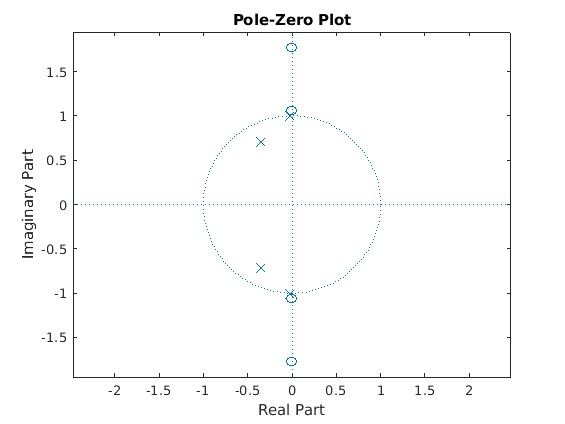
\includegraphics[scale=0.5]{root_bsf.jpg}
    \caption{Pole-Zero Plot}
    \label{fig:my_label}
\end{figure}
\subsection{Analog Bandpass Transfer Function}
The transformation is given by :
\begin{equation*}
    s_L = \frac{s^2 + \Omega_o^2 }{Bs}
\end{equation*}
Substituting the values of B and $\Omega_o$
\begin{equation*}
    s_L = \frac{s^2 + 0.8949}{3.492s}
\end{equation*}


Using the above transformation we get we get $H_{analog,BPF}$(s)  from $H_{analog,LPF}$(s)
\begin{equation*}
    \hspace*{-2cm}
    H_{analog\_BS}(s) = \frac{0.1500s^8 + 8.3311s^6 + 93.6738s^4 + 6.6722s^2 + 0.0962}{1s^8 + 2.6857s^7 + 23.9299s^6 + 38.9718s^5 + 134.1735s^4 + 34.8765s^3 + 19.1649s^2 + 1.9249s^1 + 0.6414}
\end{equation*}

\subsection{Discrete Time Filter Transfer Function}
To transform the analog domain transfer function into the discrete domain, we need to make use of the Bilinear Transformation which is given as :
\begin{equation*}
    s = \frac{1 - z^{-1}}{1 + z^{-1}}
\end{equation*}
Using  above  equation  we  get $H_{discrete,BPF}$(z)  from $H_{analog,BPF}$(s)
\begin{equation*}
    \hspace*{-2cm}
H_{discrete\_BS}(z) = \frac{0.4232z^8 - 0.0275z^7 - 1.1959z^6 + 0.0141z^5 + 1.6678z^4 + 0.0141z^3 - 1.1959z^2 - 0.0275z + 0.4232}{1z^8 - 0.1348z^7 - 1.5600z^6 + 0.0501z^5 + 1.9000z^4 - 0.0581z^3 - 0.9139z^2 - 0.0356z + 0.3903}  
\end{equation*}


\subsection{Matlab Plots}
\subsubsection{Frequency Response}
\begin{figure}[H]
\hspace*{-2.5cm}
    \centering
    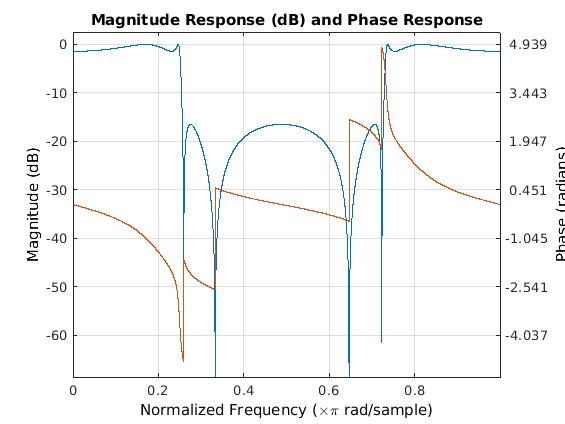
\includegraphics[width=1.5\linewidth, height=0.65\textheight]{bsf_freq.jpg}
    \label{fig:my_label}
\end{figure}

\subsubsection{Magnitude Response}
\begin{figure}[H]
\hspace*{-2.5cm}
    \centering
    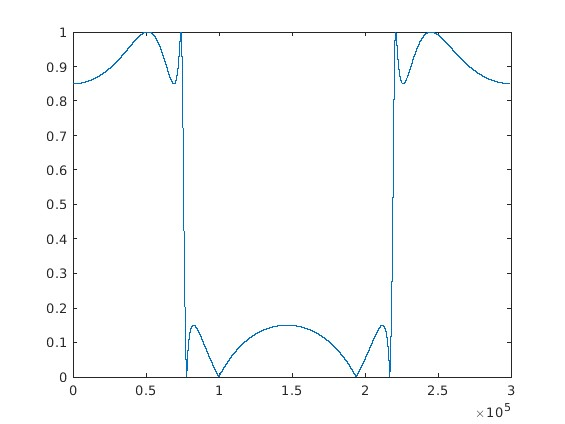
\includegraphics[width=1.5\linewidth, height=0.65\textheight]{bsf_mag.jpg}
    \label{fig:my_label}
\end{figure}

\subsubsection{Pole - Zero Plot}
\begin{figure}[H]
\hspace*{-2.5cm}
    \centering
    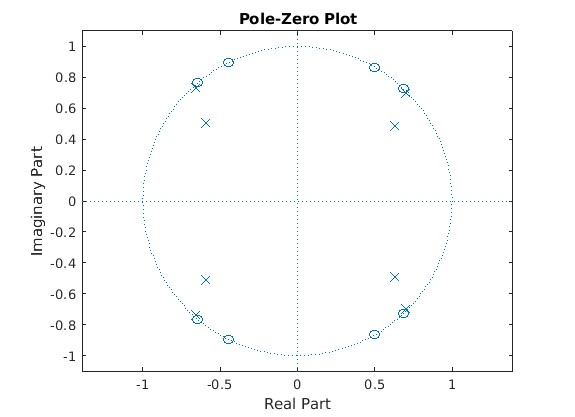
\includegraphics[width=1.5\linewidth, height=0.5\textheight]{pole_zero_bsf.jpg}
    \label{fig:my_label}
\end{figure}

As we can see, all poles of above transfer function lie within unit circle. So, the system is stable.
\newpage
\section{\textbf{Bandstop Elliptic Filter}}
\subsection{\textbf{Un-normalized Discrete Time Filter Specifications}}

\vspace{1.5em}
\noindent
The specifications of this filter are :
\begin{itemize}
    \item Stopband : \textbf{80 - 215 KHz}
    \item Passband : \textbf{0 - 75 KHz} and \textbf{220 - 300 KHz}
    \item  Transition band : \textbf{5KHz} on either side of passband
    \item  Tolerance : \textbf{0.15} in \textbf{magnitude} for both passband and stopband
    \item  Nature : Passbands and stopbands are \textbf{oscillatory} 
\end{itemize}


\subsection{Normalized Digital Filter Specifications}
Sampling rate = 600KHz\\
In the normalized frequency axis, sampling rate corresponds to 2$\pi$\\

Therefore, any frequency can be normalized as follows :
\begin{equation*}
    \omega = \frac{\Omega*2\pi}{\Omega_s}
\end{equation*}
where $\Omega_s$ is the Sampling Rate.\\

\vspace{1em}
\noindent
For the normalized discrete filter specifications, the nature and tolerances being the dependent variables remain the same while the passband and stopband frequencies change as per the above transformations. 
\begin{itemize}
    \item Stopband : \textbf{0.267 - 0.717} {$\pi$}
    \item Passband : \textbf{0 -  0.25} {$\pi$} and \textbf{0.733 - 1} {$\pi$}
    \item  Transition band : \textbf{0.0167} $\pi$ on either side of stopband
\end{itemize}



\subsection{Bilinear Transformation}
To convert to analog domain, we use the following bilinear transformation :
\begin{equation*}
    s = \frac{1 - z^{-1}}{1 + z^{-1}}
\end{equation*}
\begin{equation*}
    \Omega_{analog} = \tan (\frac{w}{2})
\end{equation*}
Applying the transformation at Band Edges we get :
\begin{table}[H]
    % Center the table
    \begin{center}
    \begin{tabular}{|c|c|}
        % To create a horizontal line, type \hline
        \hline
        % To end a column type &
        % For a linebreak type \\
        $\omega$ & $\Omega$\\
        
        \hline
            0 & 0\\
            \hline
            0.25 $\pi$ & 0.414 \\
            \hline
            0.267 $\pi$ & 0.445\\
            \hline
            0.717 $\pi$ & 2.097\\
            \hline
            0.733 $\pi$ & 2.246\\
            \hline
            $\pi$ & $\infty$\\
            \hline
        
    \end{tabular}
    \end{center}
\end{table}


Therefore, the corresponding specifications are :
\begin{itemize}
    \item Stopband :  \textbf{0.445} ($\Omega_{s1}$) - \textbf{2.097} ($\Omega_{s2}$)
    \item  Transition band : Between the passband and stopband edges
    \item Passband : \textbf{0 - 0.414}($\Omega_{p1}$) and \textbf{2.246} ($\Omega_{p2}$) \textbf{- $\infty$}
\end{itemize}


\subsection{Frequency Transformation and Relevant Parameters}
We need to convert the Band - Stop filter into a Low - Pass analog filter as we are aware of it's frequency response in order to keep equiripple passband and monotonic stopband. For that purpose we use the following frequency transformation with two parameters B and $\Omega_o$

\begin{equation*}
    \Omega_l = \frac{B\Omega}{ \Omega_o^2 - \Omega^2}
\end{equation*}

\vspace{1em}
\noindent
If we follow the convention that the passband edges are mapped to +1 and -1, the parameters, in terms of the passband edges can be obtained by solving two equations and are given by :
\begin{equation*}
    \Omega_o = \sqrt{\Omega_{p1} \Omega_{p2}} = \sqrt{0.414*2.246} = 0.964
\end{equation*}\begin{equation*}
    B = \Omega_{p2}  - \Omega_{p1} = 1.832
\end{equation*}

\begin{table}[H]
    % Center the table
    \begin{center}
    \begin{tabular}{|c|c|}
        % To create a horizontal line, type \hline
        \hline
        % To end a column type &
        % For a linebreak type \\
        $\Omega$ & $\Omega_L$\\
        
        \hline
            $0^{+}$ & $0^{+}$\\
            \hline
            0.414 ($\Omega_{p1}$) & +1 \\
            \hline
            0.445 ($\Omega_{s1}$) & 1.115\\
            \hline
            $0.946^{-}$ ($\Omega_o$) & $\infty$\\
            \hline
            $0.946^{+}$ ($\Omega_o$) & $-\infty$\\
            \hline
            2.097 ($\Omega_{s2}$)  & -1.108\\
            \hline
            2.246 ($\Omega_{p2}$) & -1\\
            \hline
            $\infty$ & $0^{-}$\\
            \hline
        
    \end{tabular}
    \end{center}
\end{table}

\vspace{1em}
\noindent
To make the filter as close to ideal as possible we choose the more stringent stopband for the lowpass filter i.e. $\Omega_{sL}$ = min($\Omega_{sL1}$ , - $\Omega_{sL2}$) = 1.108. (where $\Omega_{sL}$ stands for the stopband for the lowpass filter)

\vspace{1em}
\noindent
Therefore the analog lowpass filter specifications are as follows:
\begin{itemize}
    \item Passband Edge : 1 ($\Omega_{pL}$)
    \item Stopband Edge : 1.108 ($\Omega_{sL}$)
\end{itemize}

\subsection{Analog Elliptic Lowpass Transfer function}
As now we have $\Omega_{pL}$ and $\Omega_{sL}$, we can plug them into formula of k and k$_1$ :

\begin{equation*}
    \epsilon_p=\sqrt{(\frac{1}{0.85})^2-1}=0.6197 
\end{equation*}
\begin{equation*}
    \epsilon_s=\sqrt{(\frac{1}{0.15})^2-1}=6.5912 
\end{equation*}
\begin{equation*}
    k_1 = \frac{\epsilon_p}{\epsilon_s} = \frac{0.6197}{6.5912} = 0.0940
\end{equation*}
\begin{equation*}
    k = \frac{\Omega_{pL}}{\Omega_{sL}} = \frac{1}{1.108} = 0.9025
\end{equation*}
\begin{equation*}
N = ceil\left({\frac{K(k)\cdot K'(k_1)}{K'(k)\cdot K(k_1)}}\right) =ceil(3.3094)
\end{equation*}

From this we get N = 4 $\implies$ l=2 and r=0 and thus rounding off N, we get k = 0.9595. 
Thus we get modified value of $\Omega_{sL}$=1.0422.\\

We now just have to get the transfer function so we use equation 8,9 for getting both the things.\\
\begin{center}
Zeros are:
$z_1$=j/(0.9796*0.9595)=1.0639j\\
$z_1^*$=-1.0639j \\
$z_2$=j/(0.5891*0.9595)=1.7692j\\
$z_2^*$=-1.7692j \\
\end{center}
\begin{center}
Poles are:
$p_1$=-0.0310 + 0.9995i \\    
$p_1^*$=-0.0310 - 0.9995i \\
$p_2$=-0.3536 + 0.7071i \\
$p_2^*$=-0.3536 - 0.7071i \\
\end{center}

Pole-zero Map:
\begin{figure}[H]
    \centering
    \hspace*{-3.8cm}
    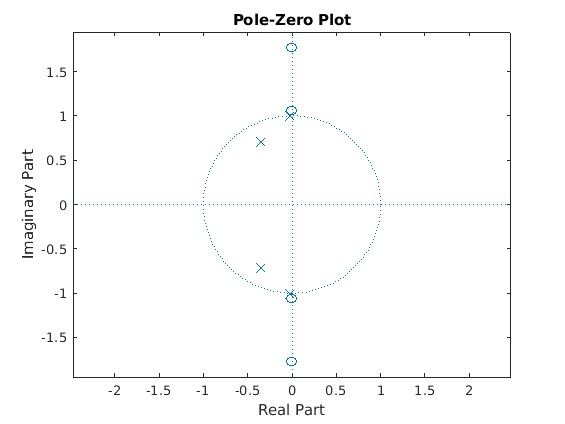
\includegraphics[scale=0.5]{root_bsf.jpg}
    \caption{Pole-Zero Plot}
    \label{fig:my_label}
\end{figure}

As N is even, we also need to account for the DC gain (which changes the normalization factor) which is $1/\sqrt(1+\epsilon^2)$, where $\epsilon$ is given by :
\begin{equation*}
    \epsilon = \sqrt{\frac{1}{(\delta_1 - 1)^2} - 1} \implies \frac{1}{\sqrt{1 + \epsilon^2}} = 1 - \delta_1
\end{equation*}
\begin{equation}
    H_{analog\_LP}(s) = \frac{0.15s^4 + 0.6392s^2 + 0.5313}{s^4 + 0.7691s^3 + 1.6689s^2 + 0.7459s + 0.6251}
\end{equation}

\subsection{Analog Bandstop Transfer Function}
The transformation is given by :
\begin{equation*}
    s_L = \frac{Bs}{s^2 + \Omega_o^2 }
\end{equation*}
Substituting the values of B and $\Omega_o$
\begin{equation*}
    s_L = \frac{1.832s}{s^2 + 0.9293}
\end{equation*}

Using the above transformation we get we get $H_{analog,BS}$(s)  from $H_{analog,LP}$(s)
\begin{equation*}
    \hspace*{-2cm}
    H_{analog\_BS}(s) = \frac{0.8500s^8 + 6.5916s^6 + 13.4861s^4 + 5.6924s^2 + 0.6339}{s^8 + 2.1861s^7 + 12.6779s^6 + 13.6600s^5 + 39.8568s^4 + 12.6942s^3 + 10.9486s^2 + 1.7544s + 0.7458}
\end{equation*}

\subsection{Discrete Time Filter Transfer Function}
To transform the analog domain transfer function into the discrete domain, we need to make use of the Bilinear Transformation which is given as :
\begin{equation*}
    s = \frac{1 - z^{-1}}{1 + z^{-1}}
\end{equation*}
Using  above  equation  we  get $H_{discrete,BS}$(z)  from $H_{analog,BS}$(s)
\begin{equation*}
\hspace*{-2cm}
    H_{discrete,BS}(z) = \frac{0.2853z^8 - 0.0557z^7 + 0.3846z^6 - 0.0890z^5 + 0.6485z^4 - 0.0890z^3 + 0.3846z^2 - 0.0557z + 0.2853}{z^8 - 0.1410z^7 - 0.1422z^6 - 0.0792z^5 + 1.3094z^4 - 0.0740z^3 - 0.1937z^2 - 0.0464z + 0.3657}   
\end{equation*}

\subsection{Matlab Plots}
\subsubsection{Frequency Response}
\begin{figure}[H]
\hspace*{-2.5cm}
    \centering
    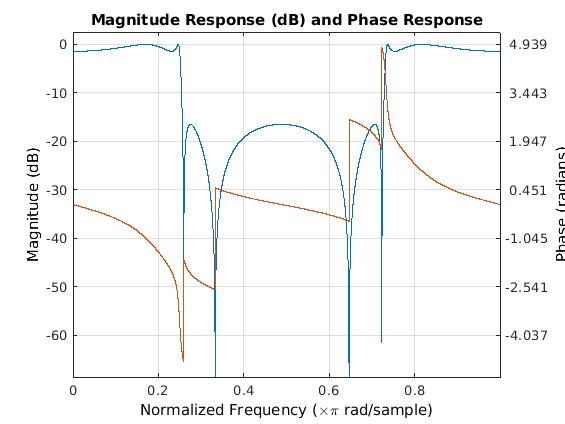
\includegraphics[width=1.5\linewidth, height=0.65\textheight]{bsf_freq.jpg}
    \label{fig:my_label}
\end{figure}

\subsubsection{Magnitude Response}
\begin{figure}[H]
\hspace*{-2.5cm}
    \centering
    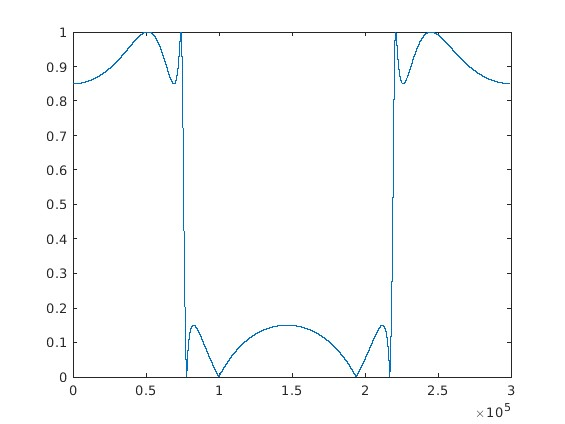
\includegraphics[width=1.5\linewidth, height=0.65\textheight]{bsf_mag.jpg}
    \label{fig:my_label}
\end{figure}

\subsubsection{Pole - Zero Plot}
\begin{figure}[H]
\hspace*{-2.5cm}
    \centering
    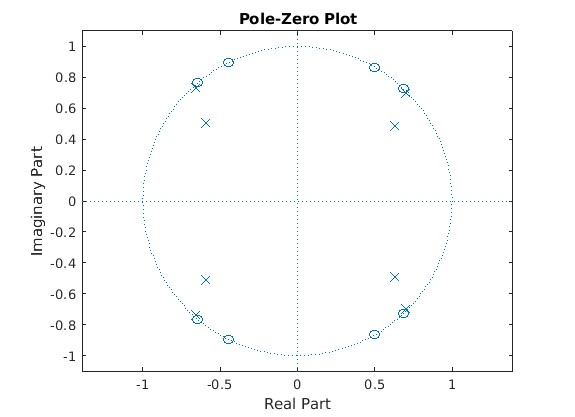
\includegraphics[width=1.5\linewidth, height=0.5\textheight]{pole_zero_bsf.jpg}
    \label{fig:my_label}
\end{figure}

As we can see, all poles of above transfer function lie within unit circle. So, the system is stable.
\newpage
\section{Final Results}
\subsection{Cascaded Transfer Funtion of Multi-Band Filter}
Our Final Transfer function has 16 zeroes and 16 poles. The coefficients of the transfer function are as follows:
\begin{table}[H]
    \centering
    \caption{Numerator Coefficients}
    \begin{tabular}{|c|c|}
        \hline
        Degree  & Coefficient \\
        \hline
        $z^{16}$ & 0.1207 \\ \hline
        $z^{15}$ & -0.0314 \\ \hline
        $z^{14}$ & -0.1769 \\ \hline
        $z^{13}$ & 0.0224 \\ \hline
        $z^{12}$ & 0.2920 \\ \hline
        $z^{11}$ & -0.0326 \\ \hline
        $z^{10}$ & -0.3121 \\ \hline
        $z^9$ & -0.0028 \\ \hline
        $z^8$ & 0.4037 \\ \hline
        $z^7$ & -0.0028 \\ \hline
        $z^6$ & -0.3121 \\ \hline
        $z^5$ & -0.0326 \\ \hline
        $z^4$ & 0.2920 \\ \hline
        $z^3$ & 0.0224 \\ \hline
        $z^2$ & -0.1769 \\ \hline
        $z^1$ & -0.0314 \\ \hline
        $z^0$ & 0.1207 \\ 
        \hline
    \end{tabular}
\end{table}

\begin{table}[H]
    \centering
    \caption{Denominator Coefficients}
    \begin{tabular}{|c|c|}
        \hline
        Degree  & Coefficient \\
        \hline
        $z^{16}$ & 1 \\ \hline
        $z^{15}$ & -0.2758 \\ \hline
        $z^{14}$ & -1.6832 \\ \hline
        $z^{13}$ & 0.2101 \\ \hline
        $z^{12}$ & 3.4348 \\ \hline
        $z^{11}$ & -0.4601 \\ \hline
        $z^{10}$ & -3.4062 \\ \hline
        $z^9$ & 0.1118 \\ \hline
        $z^8$ & 3.6880 \\ \hline
        $z^7$ & -0.1809 \\ \hline
        $z^6$ & -2.1858 \\ \hline
        $z^5$ & -0.0685 \\ \hline
        $z^4$ & 1.3882 \\ \hline
        $z^3$ & -0.0008 \\ \hline
        $z^2$ & -0.4082 \\ \hline
        $z^1$ & -0.0311 \\ \hline
        $z^0$ & 0.1427 \\ 
        \hline
    \end{tabular}
\end{table}
\subsection{Matlab Plots}
\subsubsection{Frequency Response}
\begin{figure}[H]
\hspace*{-2.5cm}
    \centering
    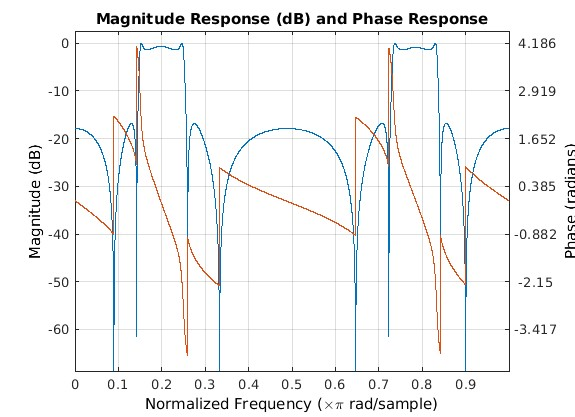
\includegraphics[width=1.5\linewidth, height=0.65\textheight]{multi_IIR_elliptic_freq.jpg}
    \label{fig:my_label}
\end{figure}

\subsubsection{Magnitude Response}
\begin{figure}[H]
\hspace*{-2.5cm}
    \centering
    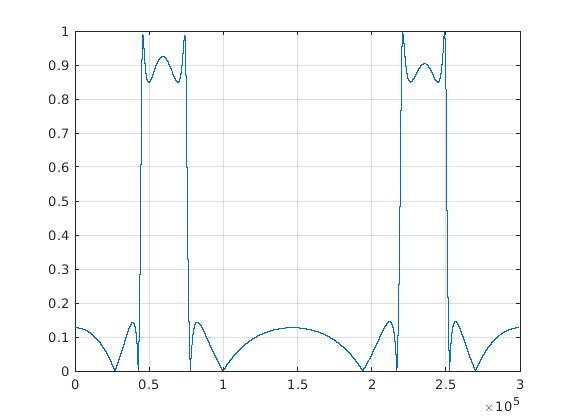
\includegraphics[width=1.5\linewidth, height=0.65\textheight]{multiband_IIR_Elliptic_mag.jpg}
    \label{fig:my_label}
\end{figure}

\subsubsection{Pole - Zero Plot}
\begin{figure}[H]
\hspace*{-2.5cm}
    \centering
    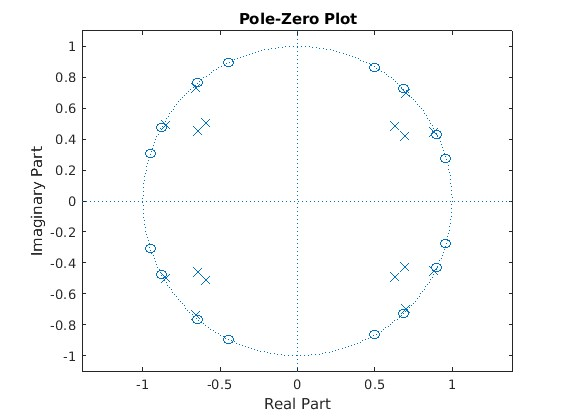
\includegraphics[width=1.5\linewidth, height=0.5\textheight]{pole_zero_final.jpg}
    \label{fig:my_label}
\end{figure}

As we can see, all poles of above transfer function lie within unit circle. So, the system is stable.

\section{Observations on Elliptical Filter Design and comparisons with Butterworth and Chebyschev}

\begin{itemize}
    \item For the same passband and stopband specifications, the order i.e. the number of resources required (which can be seen from the unit sample delays in the signal flow graph or in some sense the degree of the numerator/denominator in Z-transform), is highest for Butterworth and least for Elliptic Filter.
    \item The phase response becomes more nonlinear as we go from Butterworth to Chebyschev to Elliptic Filter. This is because the Butterworth filter has a maximally flat passband, while the Chebyschev filter has ripples in the passband and the Elliptic filter has ripples in both passband and stopband.
    \item The Elliptic Filter has the steepest transition band, followed by Chebyschev and then Butterworth. This is because the Elliptic Filter has ripples in both passband and stopband, which allows it to have a steeper transition band.
    \item The Elliptic Filter has the narrowest transition band, followed by Chebyschev and then Butterworth.
    
\end{itemize}

It's important to note that the choice of filter type depends on the specific requirements of the application, such as passband and stopband specifications, transition bandwidth, and phase linearity. Each filter type has its own advantages and trade-offs, and the appropriate filter should be selected accordingly.
\end{document}